\documentclass[12pt]{article}
\usepackage{graphicx}
\usepackage{times}
\usepackage{wasysym}
\usepackage[a4paper,left=0.8in,right=1in,top=0.5in,bottom=0.85in]{geometry}
\usepackage{tfrupee}
\usepackage{xcolor}
%% \usepackage[colorlinks]{hyperref}
%% \usepackage{url}
%% \usepackage{enumitem}
\usepackage{enumerate}
\usepackage{hyperref}
\let\iint\relax
\let\iiint\relax
\let\iiiint\relax
\let\idotsint\relax
\usepackage{lipsum}
\usepackage{fancyhdr}
\usepackage{siunitx}
\usepackage{latexsym}
\usepackage{txfonts}
\setlength{\parindent}{4em}
\setlength{\parskip}{0.5em}
\usepackage[none]{hyphenat}
%% Define variables here

\begin{document}
\definecolor{gray(x11gray)}{rgb}{0.75, 0.75, 0.75}
\definecolor{lavender(web)}{rgb}{0.9, 0.9, 0.98}
\hypersetup{urlcolor=DarkBlue}
\pagestyle{plain}
\flushleft
{\bf {CURRICULUM VITAE }}\\
%\noindent\makebox[\linewidth]{\rule{\paperwidth}{0.2pt}}
\noindent\rule{18cm}{0.2pt}
\vspace{0.05cm}
\noindent

\begin{minipage}{0.8\textwidth}
 {\bf{Suryanarayan Mondal}} \\[0.4em]
 Postdoctoral Researcher,\\
 Department of Physics,
 University of Pisa,\\
 Largo Bruno Pontecorvo 3,\\
 Pisa, Italy 56127 \\
 E-mail : suryamondal@gmail.com\\
 Mobile : +91-9732993380 \\[0.1em]
\end{minipage}% This must go next to `\end{minipage}`
\begin{minipage}{0.5\textwidth}
  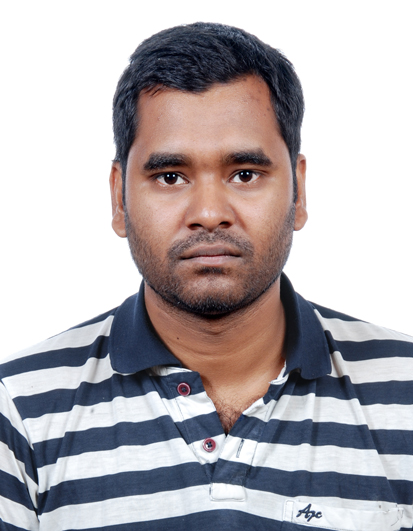
\includegraphics[width=0.45\linewidth]{./SMA454.jpg}
\end{minipage}

\vspace{0.6cm}
{\bf {Permanent Address }}\\
\begin{minipage}{0.8\textwidth}
  \vspace{0.3cm}
  Chandpur Uttarpara,\\
  Jalaberia (PO),\\
  South 24 Parganas,\\
  West Bengal--743338,\\
  India
\end{minipage}

\vspace{2cm}
\colorbox{gray!40}{\begin{minipage}{17.5cm}
\bf { EDUCATION} 
\end{minipage} }

\vspace{0.4cm}
\begin{tabular}{p{3cm} p{14cm} }

  {\emph{SSC} (2007)} & Majilpur J. M. Training School (Affiliated to West Bengal Board of Secondary Education), South 24 Parganas, West Bengal, India. \\
  & \\
  {\emph{HSC} (2009)} & Majilpur J. M. Training School (Affiliated to West Bengal Council of Higher Secondary Education), South 24 Parganas, West Bengal, India. \\
  & \\
  {\emph{BSc} (2012)} & Department of Physics, Ramakrishna Mission Vidyamandira (Affiliated to Calcutta University), Howrah, West Bengal, India.\\
  & \\
  {\emph{MSc} (2014)} & Department of Physics, Indian Institute of Technology Madras, Chennai, Tamil Nadu, India.\\
  & \\
  {\emph{PhD} (2021)} &  \emph{Thesis:} `Multiplicity of muon in $2$\,m\,$\times$\,2\,m detector and charge ratio of cosmic muon at Madurai'\\
  \vspace{0.2cm}
  & Homi Bhabha National Institute, Anushaktinagar, Mumbai, India.%% \\

\end{tabular}

\pagebreak
\vspace{0.5cm}
\colorbox{gray!40}{\begin{minipage}{17.5cm}
\bf {WORK EXPERIENCE } 
\end{minipage} }

\begin{minipage}{1.05\textwidth}
\vspace{0.4cm}
\begin{tabular}{p{3cm} p{14cm} }
  {\emph{Research Scholar}} & Tata Institute of Fundamental Research, Mumbai, Maharashtra, India 400005 (Aug 2014 -- Sept 2021)

  \begin{itemize}
  \item I was involved in India-based Neutrino
    Observatory (INO). My works were solely contributed towards
    the proposed Iron Calorimeter (ICAL) detector. This future
    underground facility is going to be dedicated for the study of the
    oscillation parameters from atmospheric neutrinos along with
    the mass ordering. Resistive Plate Chambers (RPCs) with glass
    electrodes are chosen as the sensitive detector in INO-ICAL to
    sense the signature of the muons produced in the charged-current
    interaction of neutrinos. Many prototype detector stacks were thus
    planned to study the performance of the RPCs and the electronics
    along with the data acquisition systems. I clocked a presence
    in commissioning two prototypes, gaining experience and contributing
    in some key aspects.
  \item Involved in the mechanical facets of commissioning the detectors.
  \item Formulated and implemented a easy-to-use system to estimate the
    leak tightness of RPC gaps.
  \item Developed an algorithm to fetch events with multiple tracks
    in the detector. Also isolated the events occurring due to the
    random coincidences in order to test the CORSIKA simulation.
  \item Worked in developing a method to reconstruct muon momentum
    from the data obtained in the magnetised mini-ICAL detector
    consisting of 10 layers of RPCs for the measurement of the charge
    ratio of low energy muon at the earth surface.
  \item Grasp in GEANT4, CERN-ROOT, CORSIKA software.
  \end{itemize}
  \\
  
  {\emph{Postdoctoral Researcher}} & University of Pisa, Largo Bruno Pontecorvo, Pisa, Italy 56127 (Oct 2021 --)
  
  \begin{itemize}
  \item\mbox{} I am now involved in the BelleII Collaboration, more
    specifically, in upgrade group.
    An all-pixel vertex detector is under proposal as a replacement of
    the present one. With smaller pixel size, it is capable of higher
    occupancy and vertex resolution.
    I am studying the physics performance using simulation in a
    few benchmark decay channels. 
  \end{itemize}
  
\end{tabular}
\end{minipage}

\pagebreak
\vspace{0.4cm}
\colorbox{gray!40}{\begin{minipage}{17.5cm}
\bf { STATEMENT OF RESEARCH } 
\end{minipage} }
\begin{minipage}{1.05\textwidth}
\vspace{0.4cm}
\hspace{0.5cm}
My main research interest rests in the high-energy physics, especially
in the design of the detector components, develop those, commission in
a large detector system and then extract physics out of the whole
system.

\hspace{0.5cm}
Modern particle detector setups are complex. These
setups consist of various kinds of particle detectors.
The GEANT4 simulation toolkit is proven to be effective in these
cases, simulating the properties and response of the various
components. This simulation provides a crucial role in understanding
the feasibility and the physics potential of the experiment.

\hspace{0.5cm}
Once these detector setups are commissioned, it is hard to access the
individual components. Hence much interest is given towards the
characterisation of each detector before integrating in the setup.
This process is generally repetitive and thus should require least
presence of human and minimal time. I am interested in designing
user-friendly test rigs to map the necessary traits of a detector.

\hspace{0.5cm}
As the detectors grow larger, the number of data-channels also
increases accordingly. So processing the events in order to extract
the useful information by avoiding noises (namely, track-finding)
becomes more challenging. Along with this, an algorithm to reconstruct
track parameters is required to optimise specific to the detector
setup.

\hspace{0.5cm}
The prototype detector setups, 12-layer RPC stack and magnetised
mini-ICAL, are of tracker type. Both the setups gave me plenty of
opportunity to gain knowledge on the aforesaid topics. Apart from
that I learned about the difficulties and hold-ups while commissioning
a detector setup and also gained experience of the solutions.

\hspace{0.5cm}
I had developed the leak test system from scratch and it is now
used by the whole INO collaboration. Similarly during the
commissioning of miniICAL I had solved many challenging problems,
e.g., how to unbolt the aluminium strips from the commissioned
miniICAL magnet system without dismantling the whole magnet.
These aluminium strips were bolted to the
magnet system for the smooth movement of the RPC trays in each layer,
but due to the magnetic field, the whole system shrinks beyond our
estimation, buckling those strips.
During commissioning of RPC detector at miniICAL, it was found that
few RPC can not hold pressure more than 10mm of water column, which is
necessary for stable operation of the RPC. I had temporarily
solved that button popup issue by installing suitable mylar balloon
over the RPC trays.

\hspace{0.5cm}
My concept of a FTIR detector setup to
monitor the INO gas system would have been much cheaper than a
commercial one, but could not finish due to shortage of the components.


\hspace{0.5cm}
My current involvement in the BelleII project gave me additional
opportunity to boost my knowledge in the accelerator based experiments.
Here I got to learn about the schemes and frameworks of the software tools
used along with the physics goals.
An all-pixel vertex detector is under proposal as a replacement of
the present one in the BelleII detector. With smaller pixel size, it is
capable of higher occupancy and vertex resolution.
I am studying the physics performance using simulation in a
few benchmark decay channels.

\end{minipage}

\pagebreak
\vspace{0.4cm}
\colorbox{gray!40}{\begin{minipage}{17.5cm}
\bf {LIST OF PUBLICATIONS} 
\end{minipage} }
\begin{minipage}{1.05\textwidth}
  
  \vspace{0.4cm}
  \begin{enumerate}[a.]
  \item Published:
    
    \begin{enumerate}[1.]
    \item {\bf Suryanarayan~Mondal}, V.~M.~Datar, Gobinda~Majumder, N.~K.~Mondal, K.~C.~Ravindran and B.~Satyanarayana, \emph{Leak test of Resistive Plate Chamber gap by monitoring absolute pressure}, \emph{Journal of Instrumentation, Vol} \textbf{14} (April 2019) P04009, \href{https://doi.org/10.1088/1748-0221/14/04/P04009}{DOI: 10.1088/1748-0221/14/04/P04009}
    \item {\bf Suryanarayan~Mondal}, V.~M.~Datar, Gobinda~Majumder, N.~K.~Mondal, S.~Pethuraj, K.~C.~Ravindran and B.~Satyanarayana, \emph{Study of Particle Multiplicity of Cosmic Ray Events using 2\,m\,$\times$\,2\,m Resistive Plate Chamber Stack at IICHEP-Madurai}, \emph{Experimental Astronomy}, (19 November 2020) 1--16, \href{https://doi.org/10.1007/s10686-020-09685-6}{DOI: 10.1007/s10686-020-09685-6}
    \end{enumerate} 
  \end{enumerate} 
  \begin{enumerate}[b.]
  \item Conference/Symposium
    \begin{enumerate}[1.]
    \item {\bf S.~Mondal}, V.~M.~Datar, S.~D.~Kalmani, G.~Majumder, N.~K.~Mondal and B.~Satyanarayana, \emph{Leak Rate Estimation of a Resistive Plate Chamber Gap by Monitoring Absolute Pressure in 13th Workshop on Resistive Plate Chambers and Related Detectors (RPC2016)}, \href{https://doi.org/10.1088/1748-0221/11/11/C11009}{\emph{Journal of Instrumentation, Volume } \textbf{11} (Nov 2016) C11009}
    \item {\bf Suryanarayan~Mondal}, V.~M.~Datar, S.~D.~Kalmani, G.~Majumder, N.~K.~Mondal and B.~Satyanarayana, \emph{Estimation of Leak of a Resistive Plate Chamber by Monitoring Absolute Pressure in XXII DAE High Energy Physics Symposium}, \href{https://doi.org/10.1007/978-3-319-73171-1_207}{\emph{Springer Proceedings in Physics, Volume } \textbf{203} (May 2018) 851-853}
    \item {\bf Suryanarayan~Mondal}, V.~M.~Datar, Gobinda~Majumder, N.~K.~Mondal, S.~Pethuraj, K.~C.~Ravindran and B.~Satyanarayana, \emph{Study of Particle Multiplicity by 2\,m\,$\times$\,2\,m Resistive Plate Chamber Stack at IICHEP-Madurai in XXIII DAE High Energy Physics Symposium}, \href{https://doi.org/10.1007/978-981-33-4408-2_172}{\emph{Springer Proceedings in Physics, Volume } \textbf{261} (May 2021) 1155--1158}
    \item G.~Majumder and {\bf S.~Mondal}, \emph{Design, construction and performance of magnetised mini-ICAL detector module in The 39th International Conference on High Energy Physics (ICHEP2018)}, \href{https://doi.org/10.22323/1.340.0360}{\emph{Proceedings of Science,} \textit{Volume} \textbf{340} (2019) 360}
    \item S.~Pethuraj, V.~M.~Datar, S.~D.~Kalmani, G.~Majumder, N.~K.~Mondal, {\bf S.~Mondal}, P.~Nagaraj, Pathaleswar, K.~C.~Ravindran, M.~N.~Saraf, B.~Satyanarayana, R.~R.~Shinde, Dipankar~Sil, S.~H.~Thoker, S.~S.~Upadhya, P.~Verma and E.~Yuvaraj, \emph{Measurement of Angular Distribution and Integrated Flux of Cosmic Ray Muons Using 2\,m$\times$2\,m RPC Stack at IICHEP Madurai in XXII DAE High Energy Physics Symposium}, \href{https://doi.org/10.1007/978-3-319-73171-1_205}{\emph{Springer Proceedings in Physics,} \emph{Volume} \textbf{203} (2018) 845-846}
    \item G.~Majumder, V.~M.~Datar, S.~D.~Kalmani, N.~K.~Mondal, {\bf S.~Mondal}, B.~Satyanarayana and R.~R.~Shinde, \emph{Development of a Resistive Plate Chamber with Heat Strengthened Glass in XXII DAE High Energy Physics Symposium}, \href{https://doi.org/10.1007/978-3-319-73171-1_135}{\emph{Springer Proceedings in Physics, Volume} \textbf{203} (2018) 575-578}
    \item  G.~Majumder, V.~M.~Datar, S.~D.~Kalmani, N.~K.~Mondal, {\bf S.~Mondal}, B.~Satyanarayana and R.~R.~Shinde, \emph{Development of a Resistive Plate Chamber with heat strengthened glass in 13th Workshop on Resistive Plate Chambers and Related Detectors (RPC2016)}, \href{https://doi.org/10.1088/1748-0221/11/09/C09019}{\emph{Journal of Instrumentation, Volume} \textbf{11} (2016) C09019}
    \item S.~D.~Kalmani, {\bf S.~Mondal}, R.~R.~Shinde and P.~V.~Hunagund, \emph{Some Studies Using Capillary for Flow Control in a Closed Loop Gas Recirculation System in XXII DAE High Energy Physics Symposium}, \href{https://doi.org/10.1007/978-3-319-73171-1_223}{\emph{Springer Proceedings in Physic, Volume} \textbf{203} (2018) 913-915}
    \end{enumerate}
  \end{enumerate}
\end{minipage}
\newpage

\colorbox{gray!40}{\begin{minipage}{17.5cm}
\bf {Conferences/Workshops} 
\end{minipage} }
\begin{minipage}{1.05\textwidth}
 \vspace{0.4cm}
\begin{enumerate}
  
\item Attended the course of \emph{Japan-Asia Youth Exchange program in Science (SAKURA Exchange Program in Science)} administered by Japan Science and Technology Agency and held at Osaka university, Osaka, Japan during 29--04 December, 2015. 
  
\item Attended \emph{13th Workshop on Resistive Plate Chambers and
  Related Detectors (RPC2016)} held at Ghent University, Ghent,
  Belgium during 22--26 February, 2016.\\
  {\bf{Poster Presented:}} \textsc{Leak Rate Estimation of a Resistive Plate Chamber Gap by Monitoring Absolute Pressure}.

\item Attended \emph{National Symposium on Particles, Detectors \& Instrumentation (NSPDI 2017)} held at Tata Institute of Fundamental Research, Mumbai,  India during 4-7 October, 2017. \\
  {\bf{Poster Presented:}} \textsc{Estimation of Leak of a Resistive Plate Chamber by Monitoring Absolute Pressure}.

  \item Attended \emph{XXII DAE-BRNS High Energy Physics Symposium}  held at University of Delhi, Delhi, India during 12-16 December, 2016. \\
  {\bf{Poster Presented:}} \textsc{Estimation of Leak of a Resistive Plate Chamber by Monitoring Absolute Pressure}.

\item Attended \emph{XXIII DAE-BRNS High Energy Physics Symposium}  held at IIT Madras, Chennai, India during 10-14 December, 2018. \\
  {\bf{Poster Presented:}} \textsc{Muon Multiplicity in $2$\,m\,$\times$\,2\,m RPC and comparison with CORSIKA simulation}.

\item Attended \emph{XXIV DAE-BRNS High Energy Physics Symposium}  held at NISER, Bhubaneswar, India during 14-18 December, 2020. \\
  {\bf{Poster Presented:}} \textsc{Correlation of muons arrival times from two different cosmic showers}.\\
  {\bf{Talk Presented:}} \textsc{Cosmic muon momentum spectra at Madurai}.
  
  

\end{enumerate}
\end{minipage}

\newpage
\vspace{0.6cm}
\colorbox{gray!40}{\begin{minipage}{17.5cm}
\bf {Personal Details}
\end{minipage} }

\begin{minipage}{1.05\textwidth}
\vspace{0.4cm}
\begin{tabular}{ r l}
  {\emph {Mother's Name:}} & Minakshi Jana \\[0.2cm]
  {\emph {Father's Name:}} & Lakshmi Narayan Mondal \\[0.2cm]
  {\emph {Date of Birth:}} & 12 March 1990 \\[0.2cm]
  {\emph {Place of Birth:}} & Jaynagar Majilpur, West Bengal, India \\[0.2cm]
  {\emph {Hobbies:}} & Trekking, Motorcycling \\[0.2cm]
\end{tabular}
\end{minipage} 

\end{document}
